\documentclass[11pt,a4paper]{article}

\usepackage[a4paper,left=2.0cm,right=2.0cm,top=1.55cm,bottom=1.55cm]{geometry}
\usepackage[T1]{fontenc}
\usepackage{lmodern}
\usepackage{graphicx}
\usepackage{xcolor}
\usepackage{array}
\usepackage{tabularx}
\usepackage{ragged2e}
\usepackage{enumitem}
\usepackage{fancyhdr}
\usepackage{tikz}
\usepackage{setspace}

% -------------------------------------------------
% COLOURS
% -------------------------------------------------
\definecolor{TitleBlue}{RGB}{61,103,154}

% -------------------------------------------------
% GENERAL SETTINGS
% -------------------------------------------------
\setlength{\parindent}{0pt}
\setlength{\parskip}{0pt}
\renewcommand{\arraystretch}{1.0}

\newcommand{\blueheading}[1]{%
    {\sffamily\color{TitleBlue}\fontsize{15}{18}\selectfont #1}%
}

\newcommand{\bluebigheading}[1]{%
    {\sffamily\bfseries\color{TitleBlue}\fontsize{16}{19}\selectfont #1}%
}

\newcommand{\instruction}[1]{%
    {\itshape\fontsize{10.5}{12.5}\selectfont #1}%
}

\newcommand{\answerbox}[2][]{%
    \vspace{2pt}\par
    \noindent
    {\itshape #2}\par
    \vspace{2pt}
}

% -------------------------------------------------
% HEADER / FOOTER
% -------------------------------------------------
\pagestyle{fancy}
\fancyhf{}
\renewcommand{\headrulewidth}{0pt}
\renewcommand{\footrulewidth}{0pt}

\fancyhead[L]{%
    \sffamily\bfseries\itshape\fontsize{10.5}{12}\selectfont
    COURSE NAME: Data Structure And Programing In C++ }
\fancyhead[R]{%
    \sffamily\bfseries\fontsize{10.5}{12}\selectfont
    PROJECT PROPOSAL
}
\fancyfoot[R]{%
    \itshape\fontsize{10}{12}\selectfont
    Page \thepage
}
\setlength{\headheight}{14pt}
\setlength{\headsep}{23pt}
\setlength{\footskip}{24pt}

% -------------------------------------------------
% PAGE 1
% -------------------------------------------------
\begin{document}

\vspace*{4mm}

\bluebigheading{PROJECT AND TEAM INFORMATION}

\vspace{8mm}

\blueheading{Project Title}

\vspace{1mm}

\answerbox{ClashFree: An OOP-Based Timetable Scheduler Using Graph Coloring and Constraint Satisfaction}

\vspace{8mm}

\blueheading{Student / Team Information}

\vspace{2mm}

% Team information table
% Compact 4-member layout so all members remain on Page 1.
\noindent
\begin{tabularx}{\textwidth}{|>{\RaggedRight\arraybackslash}p{0.66\textwidth}|>{\RaggedRight\arraybackslash}X|}
\hline
\begin{minipage}[t]{\linewidth}
\vspace{1.5mm}
\textit{Team ID: DSCPP-III-2026-T052}\\[-1mm]
\textit{Mentor: (Prof.) Dr.Deepak Asrani (deepakasrani.cse@geu.ac.in) Team:}
\vspace{1.5mm}
\end{minipage}
&
\begin{minipage}[t]{\linewidth}
\vspace{1.5mm}
\textit{Details}
\vspace{1.5mm}
\end{minipage}
\\
\hline
\begin{minipage}[t][3.25cm][t]{\linewidth}
\vspace{1.5mm}
\textbf{Team member 1 (Team Lead)}\\[-1mm]
\textit{(Last Name, name: student ID: email, picture):}
\vspace{2.0cm}
\end{minipage}
&
\begin{minipage}[t][3.25cm][t]{\linewidth}
\vspace{1.5mm}
\textit{Ahuja, Nishchal -- 2510380045}\\
\textit{nishchalahuja28@gmail.com}

\vspace{2mm}
\includegraphics[width=3.0cm,height=1.5cm,keepaspectratio]{nis.jpeg}
\end{minipage}
\\
\hline
\begin{minipage}[t][3.25cm][t]{\linewidth}
\vspace{1.5mm}
\textbf{Team member 2}\\[-1mm]
\textit{(Last Name, name: student ID: email, picture):}
\vspace{2.0cm}
\end{minipage}
&
\begin{minipage}[t][3.25cm][t]{\linewidth}
\vspace{1.5mm}
\textit{Bhatt, Bipul -- 2510370355}\\
\textit{bipul88bhatt08@gmail.com}

\vspace{2mm}
\includegraphics[width=3.0cm,height=1.5cm,keepaspectratio]{IMG-20251220-WA0001.jpg}
\end{minipage}
\\
\hline
\begin{minipage}[t][3.25cm][t]{\linewidth}
\vspace{1.5mm}
\textbf{Team member 3}\\[-1mm]
\textit{(Last Name, name: student ID: email, picture):}
\vspace{2.0cm}
\end{minipage}
&
\begin{minipage}[t][3.25cm][t]{\linewidth}
\vspace{1.5mm}
\textit{Singh, Mohit -- 2510370453}\\
\textit{mohit.singh.bh6@gmail.com}

\vspace{2mm}
\includegraphics[width=3.0cm,height=1.5cm,keepaspectratio]{moh.jpeg}
\end{minipage}
\\
\hline
\begin{minipage}[t][3.25cm][t]{\linewidth}
\vspace{1.5mm}
\textbf{Team member 4}\\[-1mm]
\textit{(Last Name, name: student ID: email, picture):}
\vspace{2.0cm}
\end{minipage}
&
\begin{minipage}[t][3.25cm][t]{\linewidth}
\vspace{1.5mm}
\textit{Tadiyal, Prrajval -- 2510360034}\\
\textit{prrajvaltadiyal@gmail.com}

\vspace{2mm}
 \includegraphics[width=3.0cm,height=1.5cm,keepaspectratio]{pra.jpeg}
\end{minipage}
\\
\hline
\end{tabularx}

\newpage

% -------------------------------------------------
% PAGE 2
% -------------------------------------------------

\bluebigheading{PROPOSAL DESCRIPTION}

\vspace{6mm}

\blueheading{Motivation}

\vspace{1mm}


\answerbox{%
\begin{itemize}[leftmargin=*,noitemsep,topsep=2pt,itemsep=3pt]
    \item \textbf{High Computational & Combinatorial Complexity:} Academic timetabling in modern educational institutions is a highly complex combinatorial optimization task known mathematically as the University Course Timetabling Problem (UCTP), which is proven to be NP-hard.
    \item \textbf{Vulnerability of Manual Approaches:} Traditional spreadsheet-based timetabling relies heavily on manual coordination among administrative staff, making it prone to critical hard-constraint violations such as assigning the same instructor to multiple concurrent classes, overbooking room physical capacities, or creating section overlap clashes.
    \item \textbf{Neglect of Soft-Constraint Quality:} Manual scheduling methods typically struggle to optimize soft constraints, resulting in severely fragmented student timetables with long idle gaps between sessions, unbalanced daily teaching loads for faculty members, and excessive room transitions across campus.
    \item \textbf{Institutional Scalability Bottlenecks:} As institutional enrolments grow, elective options diversify, and multi-departmental course offerings expand, manual coordination becomes computationally intractable, resource-intensive, and prone to human oversight.
    \item \textbf{Necessity of an Automated Algorithmic Solution:} Developing an automated, object-oriented software system provides a mathematically formal algorithmic framework that guarantees hard-constraint satisfaction, optimizes resource utilization, minimizes schedule fragmentation, and drastically reduces administrative preparation overhead.
\end{itemize}
}

\vspace{5mm}

\blueheading{State of the Art / Current solution}

\vspace{1mm}


\answerbox{%
\begin{itemize}[leftmargin=*,noitemsep,topsep=2pt,itemsep=3pt]
    \item \textbf{Manual & Spreadsheet-Based Planning:} Most academic departments rely primarily on manual spreadsheet software (e.g., Microsoft Excel, Google Sheets) paired with ad-hoc human review. This approach lacks real-time conflict detection, automated optimization capabilities, and computational scalability.
    \item \textbf{Commercial Off-The-Shelf (COTS) ERP Systems:} Enterprise academic management systems exist, but they operate as expensive, closed-source ``black box'' platforms. They offer limited flexibility for custom institutional rules (e.g., contiguous multi-slot practical lab allocations) and lack runtime transparency.
    \item \textbf{Absence of Benchmarking Frameworks:} Existing institutional setups rarely provide research-grade visibility or modular frameworks to evaluate, compare, and benchmark graph-coloring dynamic heuristics against exact constraint satisfaction algorithms.
\end{itemize}
}

\vspace{5mm}

\blueheading{Project Goals and Milestones }

\vspace{1mm}


\answerbox{%
\begin{itemize}[leftmargin=*,noitemsep,topsep=2pt,itemsep=3pt]
    \textbf{Core Project Goal:} Design, implement, and evaluate an efficient, object-oriented C++ software engine that models institutional timetabling as a Constraint Satisfaction Problem (CSP) via graph coloring, integrating customizable heuristic strategies and soft-constraint local search optimization engines. The project will be evaluated through three project phases (TA1-TA3) and the End Semester Theory Examination (TA4).
    \item \textbf{TA1 (Project Proposal Evaluation):} Formulate the project title, problem statement, core technical objectives, proposed object-oriented C++ architecture, curriculum subject integration, and deliver initial domain model progress.
    \item \textbf{TA2 (Mid-Term Progress Evaluation):} Build and evaluate the functional scheduling engine core, assess working code implementation, review technical progress and subject integration, conduct regular mentor interactions, and track individual contributions.
    \item \textbf{TA3 (Final Project Evaluation):} Deliver a complete working project, execute a live system demonstration, submit technical reports, demonstrate overall technical mastery, present individual contributions, and clear the oral viva voce examination.
    \item \textbf{TA4 (End Semester Theory Examination):} Comprehensive written theoretical assessment testing domain knowledge in C++ Object-Oriented Programming, Data Structures, Graph Algorithms, and Constraint Satisfaction techniques.
\end{itemize}
}



% -------------------------------------------------
% PAGE 3
% -------------------------------------------------

\blueheading{Project Approach}

\vspace{1mm}


\answerbox{%
\begin{itemize}[leftmargin=*,noitemsep,topsep=2pt,itemsep=3pt]
    \item \textbf{Mathematical Problem Formulation:} The timetabling task is mapped onto a classic Vertex Graph Coloring model $G=(V,E)$. Each vertex $v \in V$ represents a unique (course, section) lecture or lab session. An undirected edge $e=(u,v) \in E$ denotes a hard conflict (shared faculty member, room, or student cohort). Discrete time slots act as colors $c \in \{1, \dots, K\}$.
    \item \textbf{Object-Oriented Architecture & Software Patterns:} The system is designed following strict object-oriented principles. The \texttt{SchedulingStrategy} base interface uses the Strategy Design Pattern to decouple the scheduling logic, allowing seamless switching between concrete implementations: \texttt{GreedyScheduler}, \texttt{BacktrackScheduler}, and \texttt{DSATURScheduler}.
    \item \textbf{Multi-Phase Solvers & Optimization Pipeline:} The execution pipeline flows sequentially from hard-constraint resolution (graph coloring / CSP search) to soft-constraint minimization via a post-processing Local Search engine (minimizing faculty load variance and student idle gaps).
    \item \textbf{Technology Stack & Language Standards:} Developed in modern standard C++20 using standard compilers (GCC/Clang) and STL container data structures (\texttt{std::vector}, \texttt{std::unordered\_map}, \texttt{std::priority\_queue}) to maximize computational speed, ensure fine-grained memory management, and eliminate external heavyweight framework dependencies.
\end{itemize}
}

\vspace{5mm}

\blueheading{System Architecture (High Level Diagram)}

\vspace{1mm}


\answerbox{%
\centering
\vspace{1mm}
\begin{tikzpicture}[scale=0.85, transform shape, every node/.style={draw, rectangle, rounded corners=2pt, align=center, fill=TitleBlue!10, inner sep=4pt, font=\sffamily\small}]
    \node (data) at (0,1.2) {Input Data\\(CSV/JSON)};
    \node (oop) at (3.5,1.2) {OOP Data Layer\\(Entities)};
    \node (graph) at (7,1.2) {Conflict Graph\\Builder};
    \node (solver) at (7,-0.8) {Scheduling Engine\\(DSATUR / CSP)};
    \node (opt) at (3.5,-0.8) {Local Search\\Optimizer};
    \node (out) at (0,-0.8) {Export / Display\\(Grid / CSV / HTML)};

    \draw[->, thick, >=stealth] (data) -- (oop);
    \draw[->, thick, >=stealth] (oop) -- (graph);
    \draw[->, thick, >=stealth] (graph) -- (solver);
    \draw[->, thick, >=stealth] (solver) -- (opt);
    \draw[->, thick, >=stealth] (opt) -- (out);
\end{tikzpicture}
\\[2mm]
\begin{itemize}[leftmargin=*,noitemsep,topsep=2pt,itemsep=2pt]
    \item \textbf{Input Data Ingestion:} Ingests institutional CSV/JSON configuration files defining entities, availability, and resource constraints.
    \item \textbf{Domain Modeling Layer:} Instantiates C++ domain objects (\texttt{Course}, \texttt{Faculty}, \texttt{Room}, \texttt{Section}) enforcing structural integrity.
    \item \textbf{Conflict Graph Construction:} Maps non-shareable resource overlaps into an adjacency-list undirected conflict graph.
    \item \textbf{Core Scheduling Engine:} Applies strategy-based graph coloring heuristics (Greedy, Backtracking, DSATUR) to enforce hard constraints.
    \item \textbf{Post-Processing Optimizer:} Refines schedule quality using local search algorithms to minimize soft-constraint penalties.
    \item \textbf{Export & Display Exporter:} Renders clean schedule views in CLI tabular grids, CSV export files, and interactive HTML dashboards.
\end{itemize}
}

\vspace{5mm}

\blueheading{Project Outcome / Deliverables}

\vspace{1mm}

\answerbox{%
\begin{itemize}[leftmargin=*,noitemsep,topsep=2pt,itemsep=3pt]
    \item \textbf{Production C++ Scheduling Application:} A fully compiled, modular C++ application implementing Greedy, Backtracking, and DSATUR graph coloring algorithms using the Strategy Pattern.
    \item \textbf{Empirical Benchmarking & Profiling Suite:} Comprehensive benchmarking tools to evaluate dynamic saturation metrics, algorithmic runtimes, chromatic numbers, and soft-constraint violation penalties.
    \item \textbf{Multi-Format Schedule Exporters:} CLI terminal matrix renderer along with automated CSV and HTML report visualization generators for institutional deployment.
    \item \textbf{Academic Technical Documentation:} Comprehensive final report covering NP-hardness reduction proofs, heuristic algorithmic complexity analysis, and empirical performance evaluations.
\end{itemize}
}

\vspace{5mm}

\blueheading{Assumptions}

\vspace{2mm}


\answerbox{%
\begin{itemize}[leftmargin=*,noitemsep,topsep=2pt,itemsep=3pt]
    \item \textbf{Fixed Temporal Grid:} Operating schedule runs on a standard weekly grid structure consisting of 5 working days with 8 periods per day (40 total discrete time slots).
    \item \textbf{Static Resource Inputs:} Classroom capacities, faculty availability matrices, and course enrollment attributes are static and provided upfront.
    \item \textbf{Continuous Practical Block Allocation:} Laboratory and practical sessions require uninterrupted, continuous multi-slot allocations on the same day.
    \item \textbf{Negligible Travel Overhead:} Transit times between classrooms within the same campus block are assumed to be negligible between consecutive class periods.
\end{itemize}
}

\vspace{5mm}

\blueheading{References}

\vspace{1mm}


\answerbox{%
\begin{enumerate}[leftmargin=*,noitemsep,topsep=0pt]
    \item Br\'elaz, D. (1979). New methods to color the vertices of a graph. \textit{Communications of the ACM}, 22(4), 251--256.
    \item Lewis, R. (2016). \textit{A Guide to Graph Colouring: Algorithms and Applications}. Springer International Publishing.
    \item Burke, E. K., \& Petrovic, S. (2002). Recent research directions in automated timetabling. \textit{European Journal of Operational Research}, 140(2), 266--280.
\end{enumerate}
}

\end{document}